\documentclass[border=6pt]{standalone}
% Shared preamble of every figure (included by each fig*.tex)
\usepackage{fontspec}
\setmainfont{DejaVu Sans}
\setmonofont{DejaVu Sans Mono}
\usepackage{amsmath,amssymb}
\usepackage{tikz}
\usetikzlibrary{positioning,arrows.meta,fit,calc,decorations.pathreplacing,shapes.geometric,backgrounds}
\definecolor{cdata}{HTML}{4C78A8}
\definecolor{cmodel}{HTML}{F58518}
\definecolor{chead}{HTML}{54A24B}
\definecolor{cgold}{HTML}{E45756}
\definecolor{cgrey}{HTML}{9D9D9D}
\definecolor{cfull}{HTML}{B279A2}
\tikzset{
  box/.style={draw, rounded corners=2pt, align=center, inner sep=4pt, font=\small, minimum height=8mm},
  data/.style={box, fill=cdata!15, draw=cdata!80!black},
  model/.style={box, fill=cmodel!18, draw=cmodel!80!black},
  head/.style={box, fill=chead!18, draw=chead!70!black},
  note/.style={font=\footnotesize, align=center, text=black!70},
  arr/.style={-{Stealth[length=2.2mm]}, thick, black!70},
}

\usepackage{pgfplots}
\pgfplotsset{compat=1.18}
\begin{document}
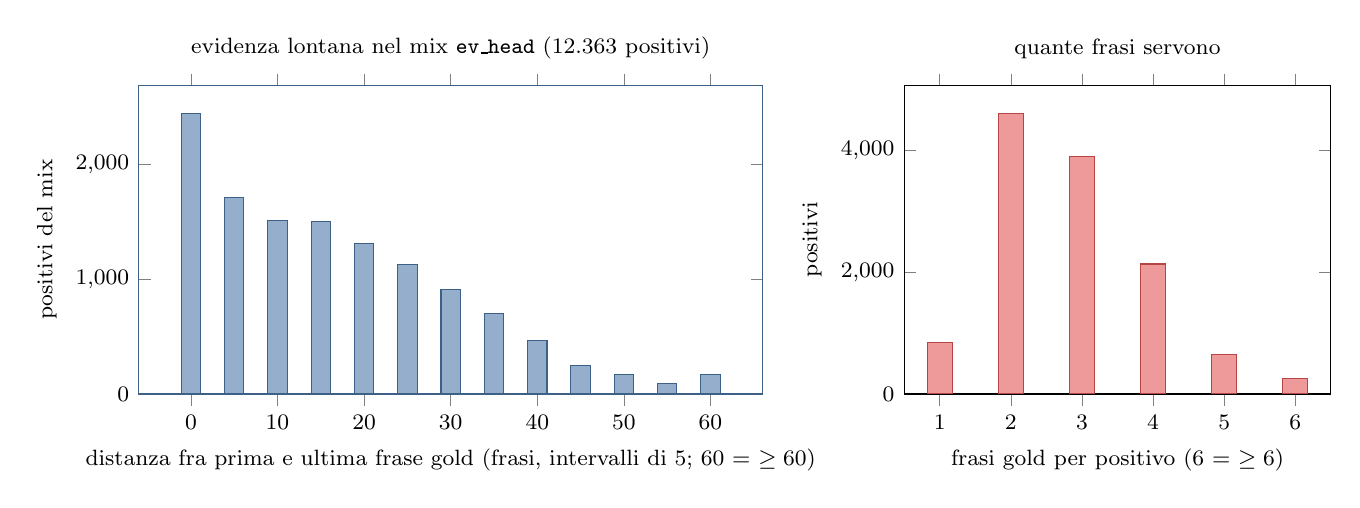
\begin{tikzpicture}
\begin{axis}[name=a, ybar, bar width=7pt, width=95mm, height=55mm, ymin=0,
  xlabel={distanza fra prima e ultima frase gold (frasi, intervalli di 5; 60 = $\ge 60$)},
  ylabel={positivi del mix}, xtick={0,10,20,30,40,50,60}, font=\footnotesize,
  title={evidenza lontana nel mix \texttt{ev\_head} (12.363 positivi)}, fill=cdata!60, draw=cdata!80!black]
\addplot[fill=cdata!60, draw=cdata!80!black] coordinates {(0,2444) (5,1714) (10,1510) (15,1504) (20,1311) (25,1126) (30,911) (35,703) (40,465) (45,247) (50,169) (55,88) (60,171)};
\end{axis}
\begin{axis}[at={(a.east)}, anchor=west, xshift=18mm, ybar, bar width=9pt, width=70mm, height=55mm, ymin=0,
  xlabel={frasi gold per positivo (6 = $\ge 6$)}, ylabel={positivi}, xtick={1,...,6}, font=\footnotesize,
  title={quante frasi servono}]
\addplot[fill=cgold!60, draw=cgold!80!black] coordinates {(1,848) (2,4601) (3,3892) (4,2131) (5,641) (6,250)};
\end{axis}
\end{tikzpicture}
\end{document}
